% Results and Discussions chapter (30% review)
% Needs in the preamble:
%   \usepackage{booktabs,graphicx,xcolor,pgfplots}
%   \pgfplotsset{compat=1.17}
% Screenshots: put the PNG files in a folder called screenshots/ next to the
% main .tex file. Until a file exists, a labelled placeholder box is shown.

\definecolor{seriesA}{HTML}{2A78D6}   % baseline / single series
\definecolor{seriesB}{HTML}{EB6834}   % custom instruction
\definecolor{inkMuted}{HTML}{52514E}
\definecolor{gridLine}{HTML}{E4E3DF}

\pgfplotsset{
  resultstyle/.style={
    axis line style={inkMuted},
    tick style={draw=none},
    major grid style={gridLine},
    tick label style={font=\small, text=inkMuted},
    label style={font=\small},
    legend style={draw=none, fill=none, font=\small},
    legend cell align=left,
  }
}

\newcommand{\screenshot}[3]{%
  \begin{figure}[h]
    \centering
    \IfFileExists{#1}{%
      \includegraphics[width=0.9\textwidth]{#1}%
    }{%
      \fbox{\parbox[c][4cm][c]{0.85\textwidth}{\centering\small
        \textbf{Screenshot placeholder}\\[1mm] Save the image as \texttt{\detokenize{#1}}\\[1mm]
        \emph{#3}}}%
    }
    \caption{#2}
  \end{figure}}

\chapter{Results and Discussions}

This chapter presents the results of the 30\% implementation. All timing
numbers were measured on the cycle-accurate Verilator simulation of the
modified Shakti C-Class core, using the hardware counters \texttt{mcycle} and
\texttt{minstret}. Every benchmark compares the output of the custom
instruction with standard RISC-V code bit for bit; all of them pass.

\section{Where the Time Goes on Baseline Shakti}

Figure~\ref{fig:profile} shows the share of execution time for one full
MobileNetV2 + GRU inference (8 frames) on the unmodified core, 31.9 billion
cycles in total.

\begin{figure}[h]
\centering
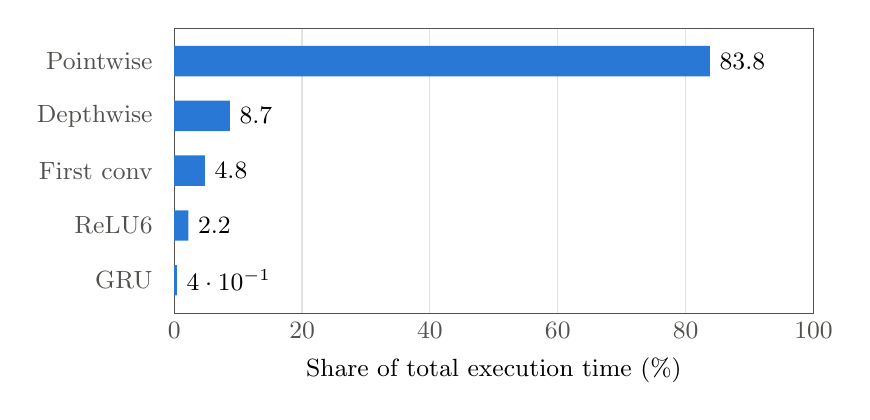
\begin{tikzpicture}
\begin{axis}[resultstyle,
  xbar, bar width=11pt, width=0.8\textwidth, height=5.2cm,
  xmin=0, xmax=100, xlabel={Share of total execution time (\%)},
  symbolic y coords={GRU,ReLU6,First conv,Depthwise,Pointwise},
  ytick=data, xmajorgrids,
  nodes near coords, nodes near coords align={horizontal},
  every node near coord/.append style={font=\small, text=black,
    /pgf/number format/fixed zerofill, /pgf/number format/precision=1},
  enlarge y limits=0.15]
\addplot[fill=seriesA, draw=none] coordinates
  {(83.8,Pointwise) (8.7,Depthwise) (4.8,First conv) (2.2,ReLU6) (0.4,GRU)};
\end{axis}
\end{tikzpicture}
\caption{Execution-time share per operation on baseline Shakti.}
\label{fig:profile}
\end{figure}

\textbf{Discussion.} Pointwise ($1\times1$) convolution takes 83.8\% of the
time, so it was the first target. The GRU takes only 0.4\%: by Amdahl's law,
accelerating it could never improve the total by more than 0.4\%. This
measurement on the target core, rather than on a PC, decided which
instructions were worth building.

\section{FDOT2 vs PFMA: Instructions vs Cycles}

Both instructions were first tested on one pointwise layer
(16$\rightarrow$96 channels, 64 pixels, 98,304 MACs).

\begin{table}[h]
\centering
\begin{tabular}{lrrrr}\toprule
Version & Cycles & Instructions & Cycles/MAC & Speedup\\\midrule
Baseline (\texttt{fmadd.s}) & 1,173,255 & 639,755 & 11.9 & 1.00$\times$\\
FDOT2.S & 1,034,125 & 338,505 & 10.5 & 1.13$\times$\\
\textbf{PFMA.S} & \textbf{702,787} & \textbf{320,362} & \textbf{7.1} & \textbf{1.67$\times$}\\\bottomrule
\end{tabular}
\caption{Single pointwise layer, baseline vs FDOT2 vs PFMA.}
\label{tab:fdot2pfma}
\end{table}

\begin{figure}[h]
\centering
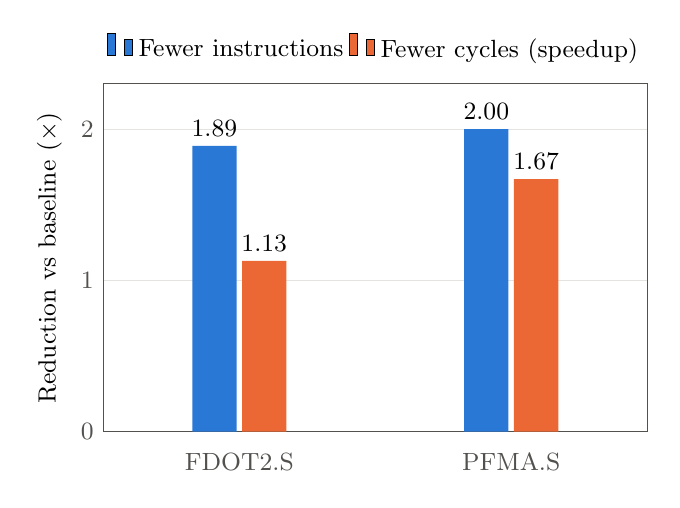
\begin{tikzpicture}
\begin{axis}[resultstyle,
  ybar, bar width=16pt, width=0.7\textwidth, height=6cm,
  ymin=0, ymax=2.3, ylabel={Reduction vs baseline ($\times$)},
  symbolic x coords={FDOT2.S,PFMA.S}, xtick=data,
  enlarge x limits=0.5, ymajorgrids,
  legend style={at={(0.5,1.03)}, anchor=south, legend columns=2},
  nodes near coords, every node near coord/.append style={font=\small,
    /pgf/number format/fixed zerofill, /pgf/number format/precision=2}]
\addplot[fill=seriesA, draw=none] coordinates {(FDOT2.S,1.89) (PFMA.S,2.00)};
\addplot[fill=seriesB, draw=none] coordinates {(FDOT2.S,1.13) (PFMA.S,1.67)};
\legend{Fewer instructions, Fewer cycles (speedup)}
\end{axis}
\end{tikzpicture}
\caption{Instruction reduction vs actual speedup.}
\label{fig:insight}
\end{figure}

\textbf{Discussion.} FDOT2 almost halved the instruction count but gave only
$1.13\times$ (Figure~\ref{fig:insight}). The two multiply-adds inside FDOT2
still run one after the other, and the FPU accepts only one operation at a
time with about 10 cycles per FMA. The real bottleneck was therefore
\emph{FMA throughput}, not instruction count. PFMA adds a second FMA unit so
two multiply-adds run in parallel, which turned the same instruction
reduction into a $1.67\times$ speedup. This was the key design decision of
the work so far.

\section{Per-Kernel Results}

\begin{table}[h]
\centering
\begin{tabular}{lccc}\toprule
Kernel & Baseline & Custom & Speedup\\\midrule
Pointwise, $K$ = 16--144 & 11.1--11.8 cyc/MAC & 6.6--7.0 & 1.69--1.70$\times$\\
Pointwise, $K$ = 320--960 & 13.8--13.9 cyc/MAC & 9.2--9.3 & 1.49--1.50$\times$\\
Depthwise $3\times3$ (incl.\ copy) & 16.99 cyc/MAC & 10.86 & 1.56$\times$\\
First conv $3\times3$, stride 2 & 18.28 cyc/MAC & 9.22 & 1.98$\times$\\
ReLU6 (PRELU6) & 14.00 cyc/elem & 3.52 & 3.98$\times$\\\bottomrule
\end{tabular}
\caption{Measured results per kernel ($K$ = number of input channels).}
\label{tab:kernels}
\end{table}

\begin{figure}[h]
\centering
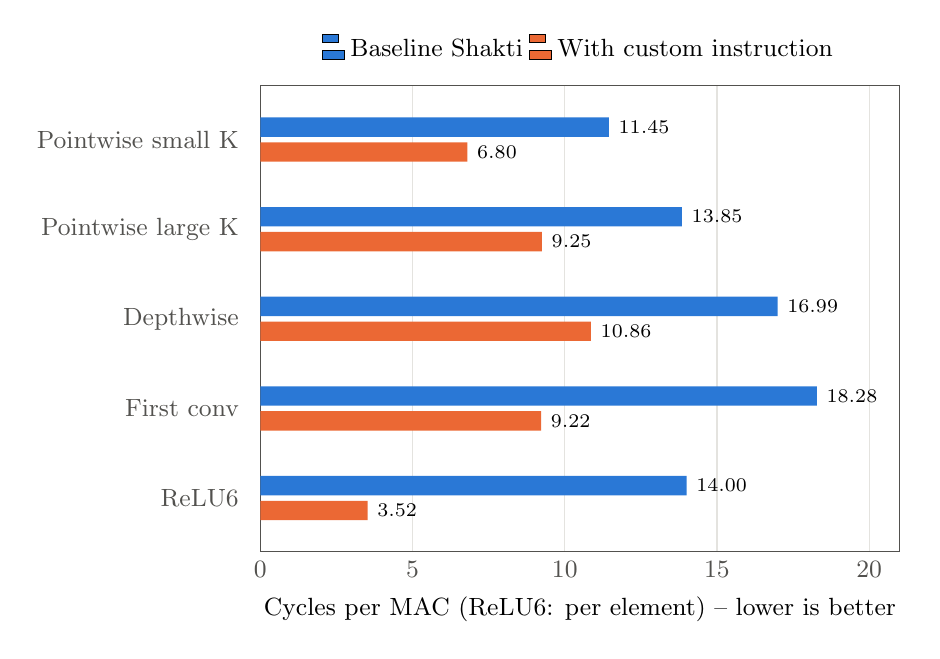
\begin{tikzpicture}
\begin{axis}[resultstyle,
  xbar, bar width=7pt, width=0.8\textwidth, height=7.5cm,
  xmin=0, xmax=21, xlabel={Cycles per MAC (ReLU6: per element) -- lower is better},
  symbolic y coords={ReLU6,First conv,Depthwise,Pointwise large K,Pointwise small K},
  ytick=data, xmajorgrids, enlarge y limits=0.15,
  legend style={at={(0.5,1.03)}, anchor=south, legend columns=2}, reverse legend,
  nodes near coords, nodes near coords align={horizontal},
  every node near coord/.append style={font=\scriptsize,
    /pgf/number format/fixed zerofill, /pgf/number format/precision=2}]
\addplot[fill=seriesB, draw=none] coordinates
  {(6.8,Pointwise small K) (9.25,Pointwise large K) (10.86,Depthwise) (9.22,First conv) (3.52,ReLU6)};
\addplot[fill=seriesA, draw=none] coordinates
  {(11.45,Pointwise small K) (13.85,Pointwise large K) (16.99,Depthwise) (18.28,First conv) (14.00,ReLU6)};
\legend{With custom instruction, Baseline Shakti}
\end{axis}
\end{tikzpicture}
\caption{Cycles per operation, baseline vs custom (pointwise values are the
middle of the measured range).}
\label{fig:cycles}
\end{figure}

\begin{figure}[h]
\centering
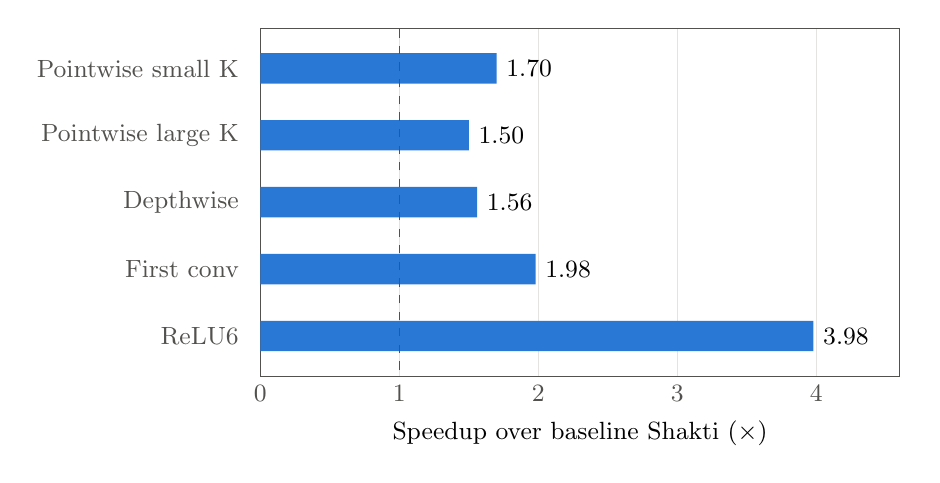
\begin{tikzpicture}
\begin{axis}[resultstyle,
  xbar, bar width=11pt, width=0.8\textwidth, height=6cm,
  xmin=0, xmax=4.6, xlabel={Speedup over baseline Shakti ($\times$)},
  symbolic y coords={ReLU6,First conv,Depthwise,Pointwise large K,Pointwise small K},
  ytick=data, xmajorgrids, enlarge y limits=0.15,
  nodes near coords, nodes near coords align={horizontal},
  every node near coord/.append style={font=\small,
    /pgf/number format/fixed zerofill, /pgf/number format/precision=2}]
\addplot[fill=seriesA, draw=none] coordinates
  {(1.70,Pointwise small K) (1.50,Pointwise large K) (1.56,Depthwise) (1.98,First conv) (3.98,ReLU6)};
\draw[inkMuted, dashed] (axis cs:1,{[normalized]-1}) -- (axis cs:1,{[normalized]5});
\end{axis}
\end{tikzpicture}
\caption{Speedup per kernel (dashed line = no speedup).}
\label{fig:speedup}
\end{figure}

\textbf{Discussion.}
\begin{itemize}
  \item \textbf{Pointwise} gains $1.69$--$1.70\times$ on small layers but only
        about $1.5\times$ on large ones. With 320--960 input channels, the
        inputs and weights (30--90\,KB) do not fit in the 16\,KB data cache,
        so both versions wait for memory. PFMA speeds up the arithmetic, not
        the memory access.
  \item \textbf{Depthwise and the first convolution} gain more per MAC because
        their inner loops are short (9 or 27 MACs), so the baseline spends
        many cycles on loop overhead. PFMA halves the number of iterations.
        The depthwise figure already includes the cost of re-arranging the
        input into pairs, so the comparison is fair.
  \item \textbf{ReLU6} gains the most ($3.98\times$): PRELU6 replaces about
        seven instructions per value with one single-cycle instruction for
        two values, because ReLU6 needs only integer comparisons on the float
        bit patterns.
\end{itemize}

\section{Whole-Model Estimate}

The cycles for one full inference were estimated by multiplying the measured
cycles per operation by the exact number of operations in MobileNetV2 + GRU
(8 frames), since simulating the full network would take several days.

\begin{figure}[h]
\centering
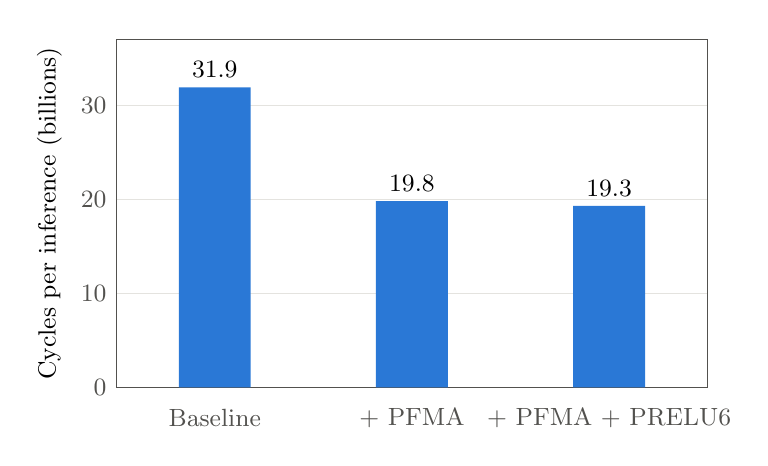
\begin{tikzpicture}
\begin{axis}[resultstyle,
  ybar, bar width=26pt, width=0.75\textwidth, height=6cm,
  ymin=0, ymax=37, ylabel={Cycles per inference (billions)},
  symbolic x coords={Baseline,+ PFMA,+ PFMA + PRELU6}, xtick=data,
  enlarge x limits=0.25, ymajorgrids,
  nodes near coords, every node near coord/.append style={font=\small,
    /pgf/number format/fixed zerofill, /pgf/number format/precision=1}]
\addplot[fill=seriesA, draw=none] coordinates
  {(Baseline,31.9) (+ PFMA,19.8) (+ PFMA + PRELU6,19.3)};
\end{axis}
\end{tikzpicture}
\caption{Estimated cycles for one MobileNetV2 + GRU inference.
Speedups: $1.61\times$ with PFMA, $1.66\times$ with PFMA + PRELU6.}
\label{fig:whole}
\end{figure}

\textbf{Discussion.} The total drops from 31.9 to 19.3 billion cycles,
a $1.66\times$ speedup. Individual kernels reach $2$--$4\times$, but the
overall figure is limited by Amdahl's law: pointwise convolution is still
about 85\% of the remaining time, and the FPU is not pipelined, so each PFMA
still waits about 10 cycles for its result. Pipelining the FPU is therefore
the next step with the largest expected gain.

\section{Verification Results}

\begin{table}[h]
\centering
\begin{tabular}{p{5cm}p{6cm}c}\toprule
Test & What it checks & Result\\\midrule
FDOT2 directed test & $[2, 1.5]\cdot[4, 3] + 0.5 = 13.0$ & Pass (\texttt{0x41500000})\\
\texttt{rv64uf/fmadd.S} (riscv-tests) & Standard FMADD unaffected after each change & Pass\\
Pointwise, depthwise, first conv benchmarks & PFMA outputs bit-identical to baseline & Pass\\
ReLU6 benchmark & PRELU6 outputs bit-identical to baseline & Pass\\\bottomrule
\end{tabular}
\caption{Verification summary (pass = \texttt{tohost} = 1).}
\end{table}

\section{Screenshots}

\screenshot{screenshots/demo_relu.png}
  {Live run of the PRELU6 benchmark on the modified Shakti core: 28,673 cycles
   (baseline) vs 7,211 cycles (PRELU6), $3.98\times$, bit-exact pass.}
  {Terminal output of \texttt{bash demo.sh relu}}

\screenshot{screenshots/git_diff_stat.png}
  {Files changed relative to the official Shakti C-Class 5.6.1 release.}
  {Output of \texttt{git diff 5.6.1 --stat --ignore-cr-at-eol -- src/}}

\screenshot{screenshots/git_diff_fpu.png}
  {RTL changes in the floating-point unit: the second FMA unit and PFMA logic.}
  {Part of \texttt{git diff 5.6.1 -- src/fpu/hardfloat/fpu\_hardfloat.bsv}}

\screenshot{screenshots/fdot2_trace.png}
  {Instruction trace (\texttt{rtl.dump}) showing the FDOT2 result 13.0
   (\texttt{0x41500000}) written to the destination register.}
  {\texttt{grep 41500000 bin/rtl.dump}}

\screenshot{screenshots/fmadd_regression.png}
  {Official \texttt{rv64uf/fmadd.S} test passing on the modified core
   (\texttt{tohost} = 1).}
  {\texttt{tohost} line from the fmadd test run}

\screenshot{screenshots/profile_report.png}
  {Profiling report of MobileNetV2 + GRU on baseline Shakti.}
  {Output of \texttt{python3 ../bench/prof\_report.py}}
